%% V1.0
%% by Gabriel Garcia, gabrcg@gmail.com
%% This is a template for Udacity projects using IEEEtran.cls

%% Be Udacious!

\documentclass[10pt,journal,compsoc]{IEEEtran}

%------------------------------------------------------

\usepackage[pdftex]{graphicx}  
\usepackage{cite}
\hyphenation{op-tical net-works semi-conduc-tor}
\usepackage[a4paper, total={6in, 9in}]{geometry}
\usepackage{amsmath}
\usepackage{booktabs}
\usepackage{caption}
\usepackage{enumitem}
\usepackage{graphicx}
\usepackage{float}
\usepackage{inconsolata}
\usepackage{listings}
\usepackage{pstricks-add}
\usepackage{siunitx}
\usepackage[most]{tcolorbox}
\usepackage{tikz}
\usepackage{epstopdf} %converting to PDF
\usepackage{hyperref}
\usepackage{makecell}
\usepackage{siunitx}
\usepackage{wrapfig}

\usetikzlibrary{shapes.geometric}

%-------------------------------------------------------
\graphicspath{{./fig/}}

%-------------------------------------------------------
\setlength{\parindent}{0in}

\lstdefinestyle{Python}{
	language        = Python,
	basicstyle      = \ttfamily,
	keywordstyle    = \color{blue},
	keywordstyle    = [2] \color{teal}, % just to check that it works
	stringstyle     = \color{green},
	commentstyle    = \color{red}\ttfamily
}

%-------------------------------------------------------
\newtcblisting[auto counter]{sexylisting}[2][]{sharp corners, 
	fonttitle=\bfseries, colframe=gray, listing only, 
	listing options={basicstyle=\ttfamily,language=Python}, 
	title=Listing \thetcbcounter: #2, #1}

%-------------------------------------------------------


\begin{document}
	
	\title{Solar Panel Soiling State Classification}
	
	\author{Shane Reynolds}
	
	\markboth{Inference project, Robotic Nanodegree, Udacity}%
	{}
	\IEEEtitleabstractindextext{%
		
		\begin{abstract}
			An abstract is meant to be a summary of all of the relevant points in your presented work. It is designed to present a high-level overview of the report, providing just enough detail to convey the necessary information The abstract may often mention a one-sentence summary of the results.  While the type of voice chosen for the paper (active or passive) may be up for debate, you should avoid the use of “I” and “me” in the report. It usually is kept to a length of 150 - 200 words. 
			Example: You should not write, “I present two different neural networks for classifying my data”. Instead, you should try to say, “Two different neural networks are used for classification”
		\end{abstract}
		
		% Note that keywords are not normally used for peerreview papers.
		\begin{IEEEkeywords}
			Robot, IEEEtran, \LaTeX, deep learning.
		\end{IEEEkeywords}}
		
		
		\maketitle
		\IEEEdisplaynontitleabstractindextext
		\IEEEpeerreviewmaketitle
		\section{Introduction}
		\label{sec:introduction}
		
		\IEEEPARstart{A}{ustralia} has the highest average solar radiation per square metre of any continent in the world. There is approximately 58 million petajoules of incident solar radiation on Austrlian soil annually - enough to meet Australia's energy demands by a multiple of 10000 \cite{Australia:2014}. Historically, Australia has used coal as its the main source of generation. Solar resources have remained largely unused - this is in line with global trends in energy consumption.
		\begin{figure}[h]
			\centering
			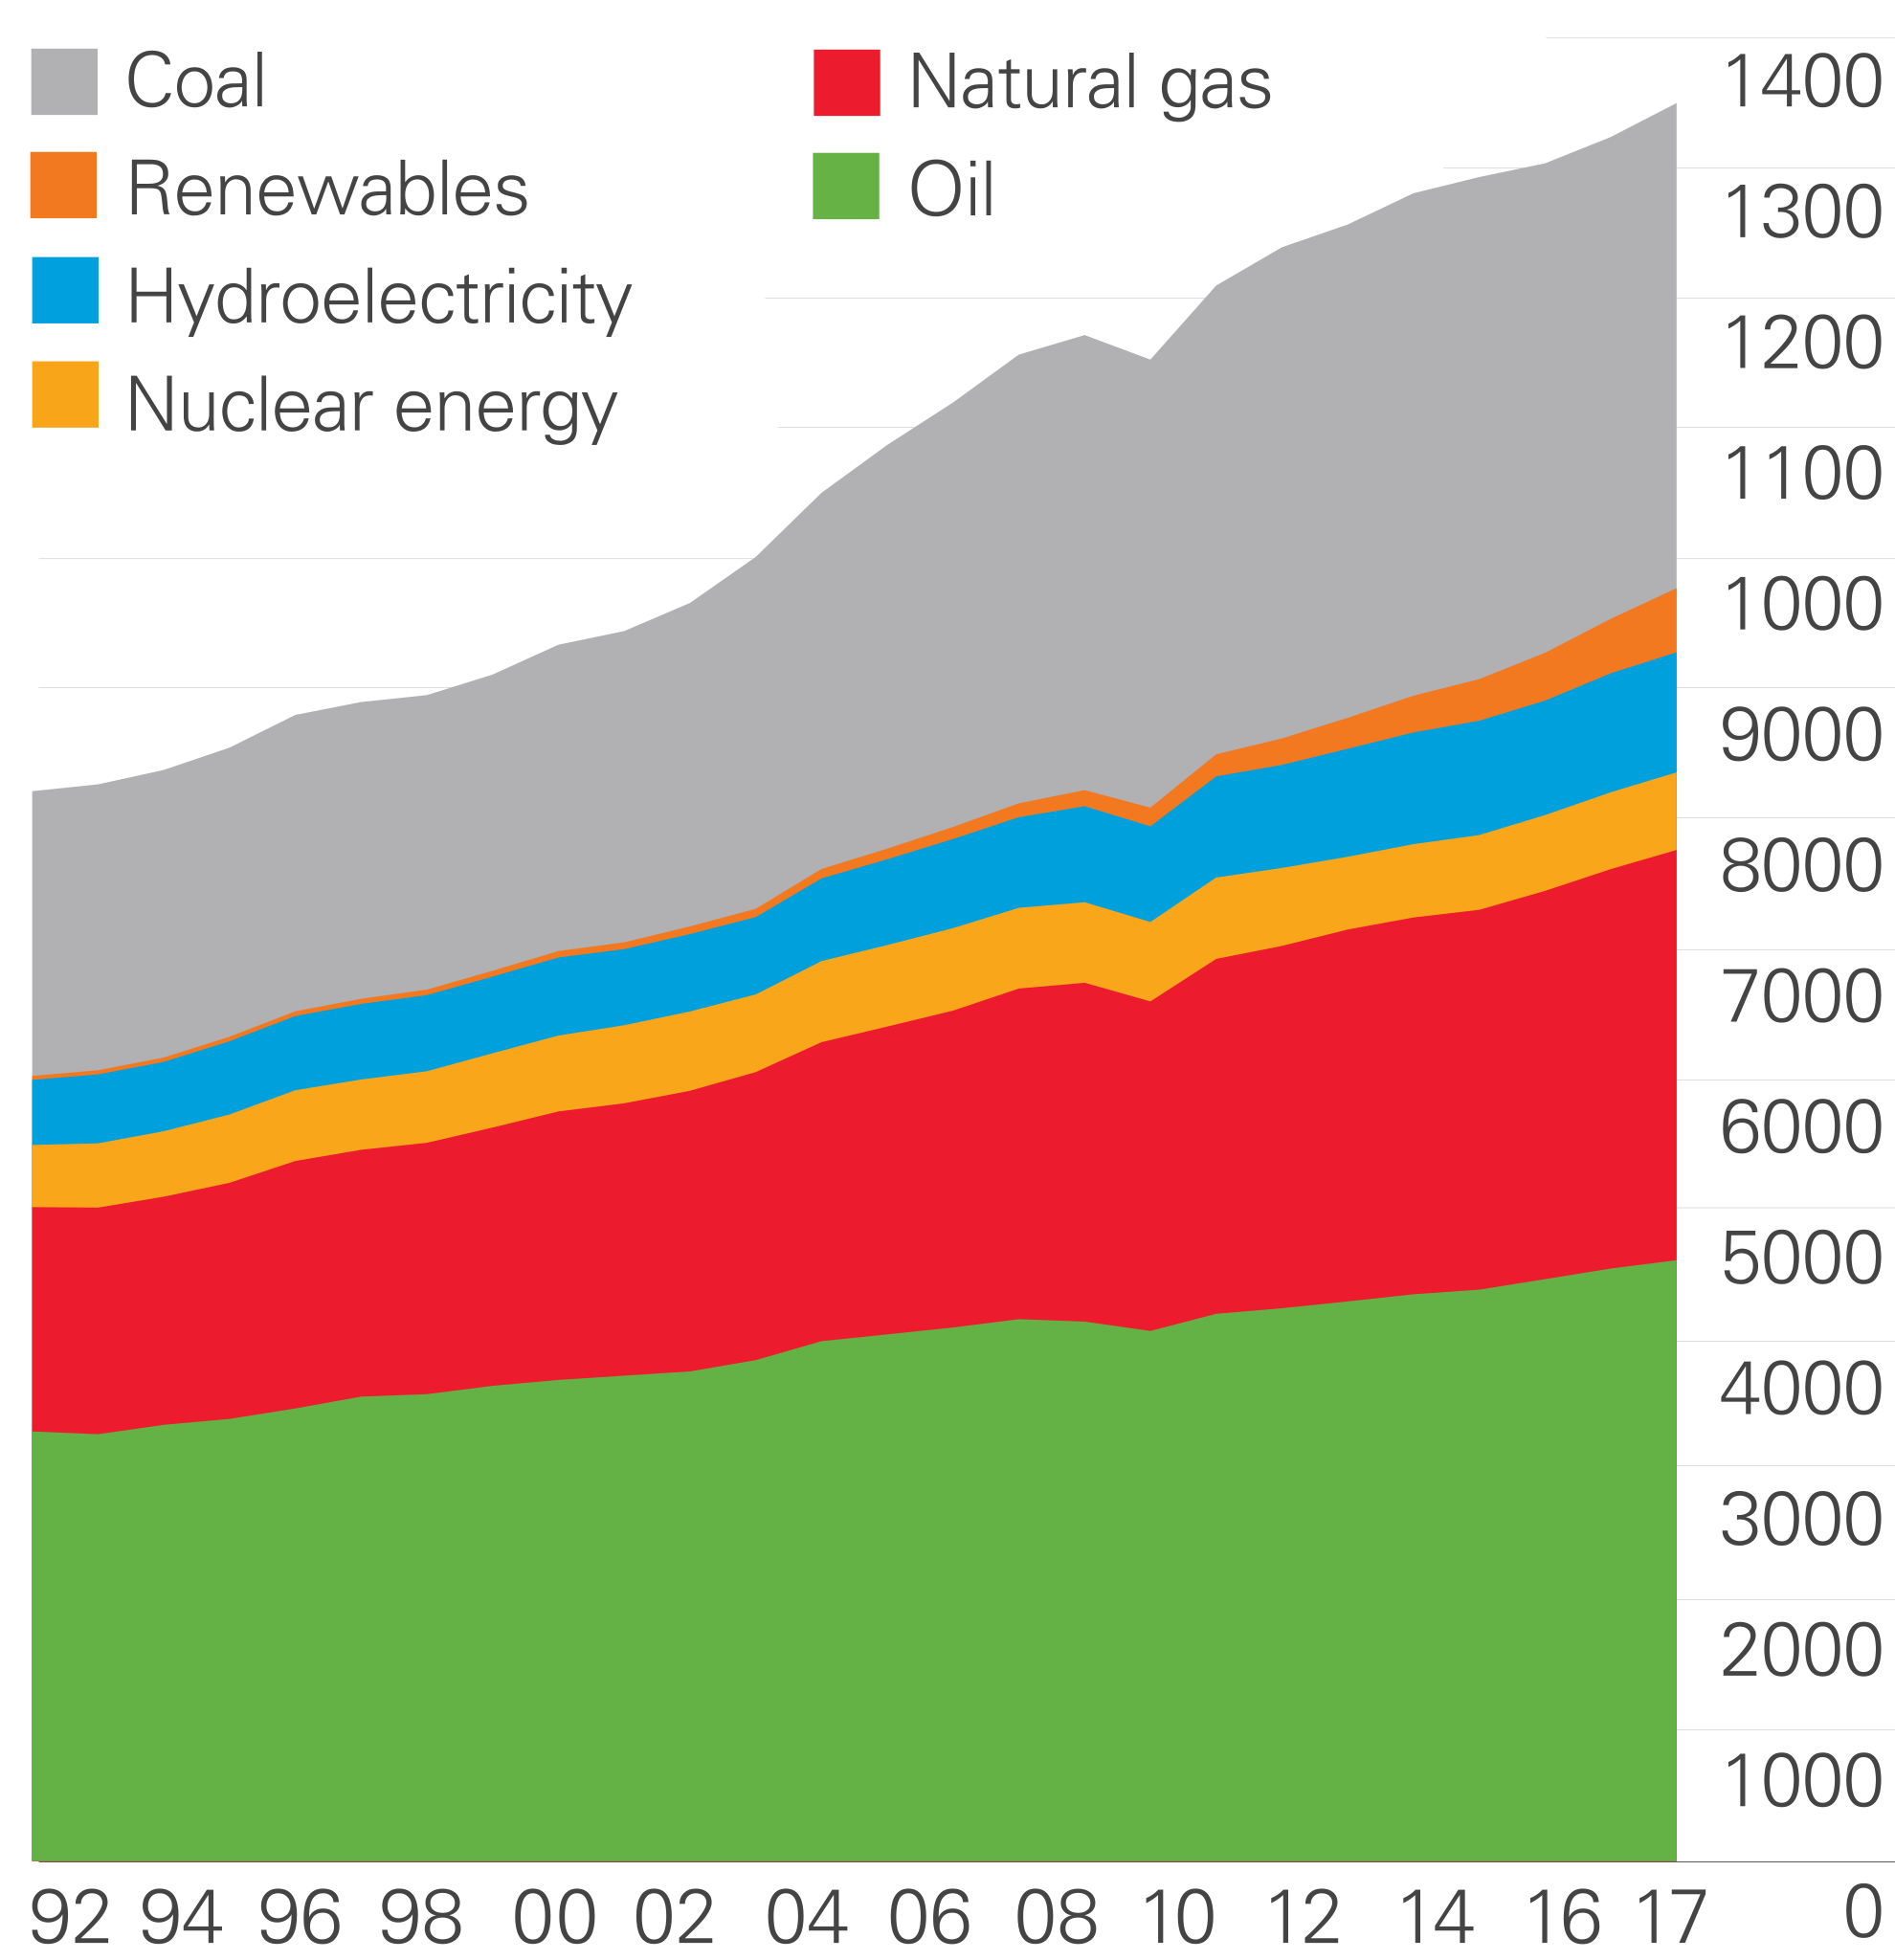
\includegraphics[scale=0.1]{globa_energy}
			\caption{Need to put a caption that will enusre the next level of text is in the next col}
		\end{figure}
		
		British Petroleum (BP) indicate coal, oil, and natural gas account for 85\% of goblal energy consumption \cite{BP:201806}. Energy from these fuels is generated from their combustion and is a major source of global greenhouse gas emissions which contribute to global warming \cite{Azapagic:2011}. In contrast, renewable sources of energy, which are comprised of wind, geothermal, solar, and biomass produce far fewer greehouse gas emissions, however, they only contribute a mere 3.5\% to global energy consumption. This is shown in a longitudinal breakdown, seen in Figure 1. The graph also shows that energy demand is increasing. If coal, oil, and natural gas remain core sources of generation then this will most likely result in greenhouse gas emissions rising, accelerating the rate of global warming. This is problematic given the well understood impacts global temperature increase has on the environment.\\
		
		The Intergovernmental Panel on Climate Change (IPCC) released a report in 2018 highlighting the link between greenhouse gas emissions and the increase in global temperatures citing human induced warming of 1$\si{\celsius}$ above pre-industrial levels in 2017, increasing at a minimum of 0.1$ \si{\celsius}$ per decade. The report forewarns of adverse environmental impact assuming maintained rates of CO2 emissions. These include an increase of 1.5$ \si{\celsius}$ above pre-industrial levels; increased frequency and intensity of heat waves; loss of biomass and a decrease in the number of species populations in climate sensitive areas; sea level rise; and food insecurity \cite{IPCC:2018}.\\ 
		
		Fortunately, the solar power industry is growing in Australia. As of September 2018, Australia had over 10131$\si{\mega\watt}$ of installed PV solar power. Approximately, 3366$\si{\mega\watt}$ were installed in the preceding 12 months \cite{APVI:2018}. In fact, the Australian renewable energy industry is on track to install more than 10$\si{\giga\watt}$ of new solar power during 2018 and 2019 - a rate which, if sustained, would see Australian generation reach 50\% renewables by 2025 \cite{Baldwin:2018}.\\
		
		Generation from large- and mid-sized solar arrays face the unique maintenance challenge of keeping the solar panels free from soiling. Soilng comes in the form of an accumutaion of dust, pollen, leaves, bird droppings or snail trails \cite{Maghami:2016}. An IBM research lab in 2018 demonstrated that Fully Convolutional Neural Networks can be used to help determine the soiling states of solar panels. Approximately 45000 images of solar panels in various states of soiling were collected. Trained models were successfully able to use object detection to locate the soiled regions of solar panels. Additionally, models could classify types of soiling, and provide an estimate of the power loss experienced by an individual panel \cite{Mehta:2018}.\\
		
		This paper proposes the use of a CNNs to classify images of solar panels as soiled or clean. A simple classification network like this could be used to set up an automatic visual inspection system, using drones equipped with RGB cameras, to determine soiling states for large solar arrays. This is of interest as it would allow scheduling of cleaning routines for maintenance cost optimisation. Cost savings would be realised reductions in labour required for manual visual inspections. Additionally, data could be used to determine optimal cleaning sequences for maximum power efficiency.\\
		
		\section{Background / Formulation}
		A Convolutional Neural Network (CNN) is a class of artificial neural network, which has an underlying architecture suited to learning shapes, edges, and colours in images. The main feature of a CNN is a convolving filter, which can be thought of as a small patch which slides over the image allowing model weights to be shared for different sections of the image. An example of this can be seen in Figure 2.\\
		\begin{figure}[h]
			\centering
			\includegraphics[scale=0.35]{CNN}
			\caption{An example of a convolutional layer - the small panel is convolved across the image producing the output (shown in blue).}
		\end{figure}
		
		CNNs are recognised as state-of-the-art methods for image classification, as seen in models such as GoogleNet \cite{Szegedy:2014}, ResNet \cite{He:2015}, and VGG \cite{Simonyan:2015}. Of course, recent CNNs, such as VGG, are very deep and contain a significant number of weights. This has two well understood effects:
		\begin{enumerate}
			\item High numbers of model weights requires more data to ensure that the model is adequately trained;
			\item Deep models dramatically increase the computation required for classification, making inference slower \cite{Cansiani:2017}.
		\end{enumerate}
		
		The second point is demonstrated pictorially, shown in Figures 3 and 4.
		
		\begin{figure}[h]
			\centering
			\includegraphics[scale=1]{tradeoff}
			\caption{This image shows the trade off between the number of operations, accuracy, and number of parameters}
		\end{figure}
		
		\begin{figure}[h]
			\centering
			\includegraphics[scale=1]{tradeoff_2}
			\caption{This image compares the inference times of different model architectures}
		\end{figure}
		
		
		\clearpage
		\begin{figure*}[h]
			\centering
			\includegraphics[scale=1]{googlenet_arch}
			\caption{text}
		\end{figure*}
		\clearpage
		
		Given the lack of available image data for soiled solar panels, a model with too many parameters poses a risk of underfitting. This would yield poor classification results. Additionally, inference needs to be fast. A trained model deployed on a drone, used for soiling classification of a large solar panel array, will need to be able to process image data quickly. To help ensure performance requirements are met, some minimum benchmarks were perscribed for a secondary data set, not related to the solar panel classification problem. These include:
		\begin{enumerate}
			\item A hurdle rate of 75\% accuracy on model classification
			\item An inference speed of less than 10$\si{\milli\second}$ for a single image, given model deployment on [WHAT HARDWARE IS THIS]
		\end{enumerate}
		
		Googlenet was selected as the best model architecture Ready and available off the shelf that needed little to no development and amoung the state of the art model selections seemed to provide the best balance between model accuracy and inference time. It must be noted that this is most likely not the most optimal model - there is most likely some application specific model which would deliver superior performance and speed - this is similar to design choices when looking at embedded systems. For rapid system development the additional time and cost spent developing optimised systems means that the product may be redundant by the time that it is ready for release.
			
		\section{Data Acquisition}
		Image data was collected for threee distinct categories: soiled solar panels, clean solar panels, and images with no solar panels. Data was aquired from Google image searches which was automated used a Python module called XX. Keywords to search for each category can be seen in Table 1.
		\begin{table}[h]
			\centering
			\caption{text}
			\begin{tabular}{ll}
				\toprule
				\textbf{Classification Category} & \textbf{Keywords} \\
				\midrule
				Clean Solar Panels & \textit{Clean Solar Panels}\\
				 & \\
				Soiled Solar Panel & \textit{Dirty Solar Panel} \\
				 & \textit{Dusty Solar Panel} \\
				  & \\
				No Solar Panel & \textit{Roof} \\
				 & \textit{Rooftops} \\
				\bottomrule
			\end{tabular}
		\end{table}
		
		Each keyword search from the module returned 100 images, however, not all returned images were suitable and some were discarded during a manual review. This left 161 images for the No Solar Panel category; 102 images for the Soiled Solar Panel category; and 39 images for the Clean Solar Panel category. The final image sets were resized to 256$\times$256 - this introduced some distortion, due to unequal scaling, for those images that did not have square dimensions. Distortion could be avoided by image cropping, however, this would have added further complexity pre-processing.
		\begin{figure}[h]
			\centering
			\frame{\includegraphics[scale=0.5]{clean}}
			\caption{Example of an image of clean solar panels.}
		\end{figure}
		
		\begin{figure}[h]
			\centering
			\frame{\includegraphics[scale=0.5]{dirty}}
			\caption{An example of an image of soiled solar panels.}
		\end{figure}
		
		\begin{figure}[h]
			\centering
			\frame{\includegraphics[scale=0.5]{no_solar}}
			\caption{An example of an image of no solar panels.}
		\end{figure}
		
		Samples of images collected for the Clean Solar Panel, Soiled Solar Panel, and No Solar Panel can be seen in Figures 6, 7, and 8, respectively. The number of images for each class were doubled using a trick in which images are flipped from left to right and added back to the class. The final number of images are as follows:
		\begin{itemize}
			\item \textbf{Clean solar panels:} 78
			\item \textbf{Dirty solar panels:} 204
			\item \textbf{No solar panels:} 322
		\end{itemize}
			
		\section{Results}
		\subsection{Trial Data}
		Training the Googlenet model on the trail data set, over 3 epochs with a batch size of XX, resulted in a 
		\begin{figure}[h]
			\centering
			\includegraphics[scale=0.3]{trial_data_model_train}
			\caption{text}
		\end{figure}
		
		The model was evaluated using a set of test data which the model had not been exposed to which resulted in an accuracy of XX\%. Further, the inference speed of the model was 
		
		\subsection{Solar Panel Data}
		Training the Googlenet model on the solar panel data set, over XX epochs with a batch size of XX, resulted in a 
		\begin{figure}[h]
			\centering
			\includegraphics[scale=0.3]{googlenet_train_img}
			\caption{text}
		\end{figure}
		
		This is typically the hardest part of the report for many. You want to convey your results in an unbiased fashion. If you results are good, you can objectively note this. Similarly, you may do this if they are bad as well. You do not want to justify your results here with discussion; this is a topic for the next session. 
		Present the results of your robotics project model and the model you used for the supplied data with the appropriate accuracy and inference time
		For demonstrating your results, it is incredibly useful to have some charts, tables, and/or graphs for the reader to review. This makes ingesting the information quicker and easier.
			
		\section{Discussion}
		This is the only section of the report where you may include your opinion. However, make sure your opinion is based on facts. If your results are poor, make mention of what may be the underlying issues. If the results are good, why do you think this is the case? Again, avoid writing in the first person (i.e. Do not use words like “I” or “me”). If you really find yourself struggling to avoid the word “I” or “me”; sometimes, this can be avoid with the use of the word “one”. As an example: instead of : “I think the accuracy on my dataset is low because the images are too small to show the necessary detail” try: “one may believe the accuracy on the dataset is low because the images are too small to show the necessary detail”. They say the same thing, but the second avoids the first person. 
		Reflect on which is more important, inference time or accuracy, in regards to your robotic inference project.
			
		\section{Conclusion / Future work}
		This section is intended to summarize your report. Your summary should include a recap of the results, did this project achieve what you attempted, and is this a commercially viable product? 
		For Future work,address areas of work that you may not have addressed in your report as possible next steps. For future work, this could be due to time constraints, lack of currently developed methods / technology, and areas of application outside of your current implementation. Again, avoid the use of the first-person.
			
		\bibliography{my_bib}
		\bibliographystyle{ieeetr}
			
\end{document}